\documentclass{article}
\usepackage{amsmath}
\usepackage{amsfonts}
\usepackage{tikz}
\usepackage{graphicx}
\usepackage{listings}

\begin{document}

\section*{Student Information}
Name: Batuhan Akçan \\
ID: 2580181 \\

\section*{Answer 1}
\subsection*{a)}
The sample mean is:\vspace{0.2cm}\\ $\overline{X} = \frac{\left(8.4+7.8+6.4+6.7+6.6+6.6+7.2+4.1+5.4+6.9+7.0+6.9+7.4+6.5+6.5+8.5\right)}{16} = 6.81$\vspace{0.2cm}\\
The sample standard deviation is:\vspace{0.2cm}\\
$s = \sqrt{\frac{\Sigma (x_i-\overline{x})^2}{n-1}} = \sqrt{\frac{(8.4-6.81)^2+(7.8-6.81)^2+...+(8.5-6.81)^2}{16-1}} = 1.06$\vspace{0.2cm}\\
With $\alpha = 0.02$ and $d.f. = n-1 = 15$, according to Student's T-distribution table, $t_{\alpha/2} = t_{0.01} = 2.6$\vspace{0.2cm}\\
The confidence interval is:\vspace{0.2cm}\\
$\overline{X} \pm t_{\alpha/2}\frac{s}{\sqrt{n}} = 6.81 \pm 2.6\cdot \frac{1.06}{4} = [6.12,7.50]$.
\subsection*{b)}
We will test the null hypothesis $H_0: \mu = 7.5$ against a left-tail alternative $H_A: \mu < 7.5$. Since the standard deviation is unknown, and we have only one sample, we will use the one-sample T test for mean.\vspace{0.2cm}\\
$t = \frac{\overline{X}-\mu_0}{s/\sqrt{n}} = \frac{6.81-7.5}{1.06/4} = -2.60$\vspace{0.2cm}\\
With $\alpha = 0.05$ (we don't divide by 2 because it is one-sided), $d.f. = 16-1 = 15$, according to Student's T-distribution table, $-t_{0.05} = -1.75$.\vspace{0.2cm}\\
Since $-2.60 < -1.75$, we reject the null hypothesis, i.e., we can claim that the improvement is effective (there is a significant reduction in the gasoline consumption).
\subsection*{c)}
We will calculate the P-value. The t-statistic for new $\mu_0$ is:\vspace{0.2cm}\\
$t = \frac{\overline{X}-\mu_0}{s/\sqrt{n}} = \frac{6.81-6.5}{1.06/4} = 1.17$\vspace{0.2cm}\\
With $d.f. = 15$, according to Student's T-distribution table, $P = P\{t \leq t_{obs}\} = P\{t \leq 1.17\} = F_v(1.17) > 0.1$. (the $\leq$ symbol is due to the fact that the alternative hypothesis is left-tail.)\vspace{0.2cm}\\
Since $F_v(1.17) > 0.1$, we can immediately accept $H_0$.

\section*{Answer 2}
\subsection*{a)}
$H_0: \mu = 5000\;$against a right-tail alternative$\; H_A: \mu > 5000.$\\
Ali's claim should be considered as the null hypothesis.
\subsection*{b)}
Since the standard deviation is known and we have only one sample, we will use the one-sample Z-test for mean.\vspace{0.2cm}\\
$Z = \frac{\overline{X}-\mu_0}{\sigma/\sqrt{n}} = \frac{5500-5000}{2000/\sqrt{100}} = 2.5$\vspace{0.2cm}\\
With $\alpha = 0.05$ (we don't divide by 2 because it is one-sided), according to Standard Normal Distribution table, $z_{0.05} = p_{0.95} = 1.65$.\vspace{0.2cm}\\
Since $2.5 > 1.65$, we reject the null hypothesis, i.e., Ahmet can claim that there is an increase in the rent prices.
\subsection*{c)}
$P = P\{Z \geq 2.5\} = 1 - \phi(2.5) = 1 - 0.994 = 0.006$.\vspace{0.2cm}\\
Since $0.006 < 0.01$, we can immediately reject the null hypothesis, i.e., we can immediately accept Ahmet's claim.
\subsection*{d)}
Let X = Ankara and Y = Istanbul.
We will test the null hypothesis $H_0: \mu_X - \mu_Y = 0$ against a left-tail alternative $H_A: \mu_X - \mu_Y < 0.$
Since the standard deviation is known and we have 2 samples, we will use the two-sample z-test for means.\vspace{0.2cm}\\
$Z = \frac{\overline{X}-\overline{Y}-D}{\sqrt{\frac{\sigma_x^2}{n}+\frac{\sigma_y^2}{m}}} = \frac{5500 - 6500 - 0}{\sqrt{\frac{2000^2}{100}+\frac{3000^2}{60}}} = -2.29$\vspace{0.2cm}\\
With $\alpha = 0.01$ (we don't divide by 2 because it is one-sided), according to Standard Normal Distribution table, 
$-z_{0.01} = -p_{0.99} = -2.33$ \vspace{0.2cm}\\
Since $-2.29 > -2.33$, we can accept the null hypothesis, i.e., the average prices in Ankara are the same as the average prices in Istanbul.\vspace{1.5cm}\\

\section*{Answer 3}
We will test the null-hypothesis $H_0: $\;"the number of rainy days in Ankara is independent from the season" against the alternative hypothesis $H_A: $\;"the number of rainy days in Ankara is dependent to the season".
We will use the Chi-square test for independence. The contingency table for observed counts is:\vspace{0.2cm}\\

\begin{center}
\begin{tabular}{ c|c|c|c|c|c }
 $Obs(i,j)=n_{ij}$ & Winter & Spring & Summer & Autumn & $n_{i\cdot}$  \\
 \hline
 Rainy & 34 & 32 & 15 & 19 & 100 \\ 
 \hline
 Non-Rainy & 56 & 58 & 75 & 71 & 260 \\ 
 \hline
 $n_{\cdot j}$ & 90 & 90 & 90 & 90 & 360 \\ 
 \hline
\end{tabular}
\end{center}\vspace{0.2cm}
\hspace{-0.1cm}
$\widehat{Exp}(1,1) = \widehat{Exp}(1,2) = \widehat{Exp}(1,3) = \widehat{Exp}(1,4) = \frac{90\cdot 100}{360} = 25$\vspace{0.2cm}\\
$\widehat{Exp}(2,1) = \widehat{Exp}(2,2) = \widehat{Exp}(2,3) = \widehat{Exp}(2,4) = \frac{90\cdot 260}{360} = 65$\vspace{0.2cm}\\
Hence, the contingency table for expected counts is:\vspace{0.2cm}\\

\begin{center}
\begin{tabular}{ c|c|c|c|c|c }
 $\widehat{Exp}(i,j)=\frac{(n_{i\cdot})(n_{\cdot j})}{n}$ & Winter & Spring & Summer & Autumn & $n_{i\cdot}$  \\
 \hline
 Rainy & 25 & 25 & 25 & 25 & 100 \\ 
 \hline
 Non-Rainy & 65 & 65 & 65 & 65 & 260 \\ 
 \hline
 $n_{\cdot j}$ & 90 & 90 & 90 & 90 & 360 \\ 
 \hline
\end{tabular}
\end{center}\vspace{0.2cm}
\hspace{-0.1cm}
$\chi_{obs}^2 = \frac{(34-25)^2}{25} + \frac{(32-25)^2}{25} + \frac{(15-25)^2}{25} + \frac{(19-25)^2}{25} + \frac{(56-65)^2}{65} + \frac{(58-65)^2}{65} + \frac{(75-65)^2}{65} + \frac{(71-65)^2}{65} = 14.73$\vspace{0.2cm}\\

With $(4-1)(2-1) = 3$ degrees of freedom, according to Chi-Square table, we find that $0.001 < P < 0.005$. Since $P < 0.01$, we will reject the null-hypothesis, i.e., the number of rainy days in Ankara is dependent to the season.
\vspace{4.5cm}\\

\section*{Answer 4}
\subsection*{Code:}
\lstset
{tabsize=2}
\begin{lstlisting}
pkg load statistics

input = [34,32,15,19; 56,58,75,71];

i = 1;
n_j = [];
while (i<=columns(input))
	j = 1;
	summ = 0;
	while (j<=rows(input))
		summ += input(j,i);
		j++;
	endwhile
	n_j = horzcat(n_j, summ);
	i++;
endwhile

i = 1;
n_i = [];
while (i<=rows(input))
	j = 1;
	summ = 0;
	while (j<=columns(input))
		summ += input(i,j);
		j++;
	endwhile
	n_i = horzcat(n_i, summ);
	i++;
endwhile

exp_cont_table = [];
i = 1;
while (i<=rows(input))
	j = 1;
	tmp = [];
	while (j<=columns(input))
		res = n_i(i) * n_j(j) / sum(n_i);
		tmp = horzcat(tmp, res);
		j++;
	endwhile
	exp_cont_table = vertcat(exp_cont_table, tmp);
	i++;
endwhile

chi2 = 0;    	% chi-square value
i = 1;
while (i<=rows(input))
	j = 1;
	while (j<=columns(input))
		chi2 += power(input(i,j)-exp_cont_table(i,j), 2) / exp_cont_table(i,j);
		j++;
	endwhile
	i++;
endwhile

df = (rows(input)-1)*(columns(input)-1);
p_value = 1 - chi2cdf(chi2, df);  % p-value

\end{lstlisting}

\vspace{3cm}
Note: The screenshot is in the next page. The chi-square value and the p-value can be seen at the end of the screenshot.

\subsection*{Screenshot:}
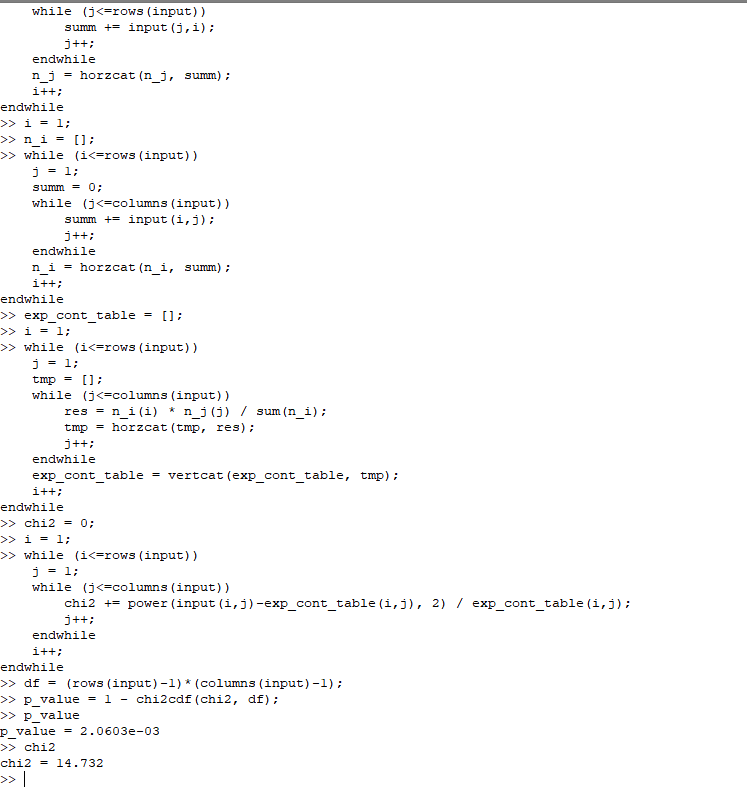
\includegraphics[width=1.5\textwidth]{code.png} 














\end{document}